\documentclass[10pt]{article}
\usepackage[T1]{fontenc}
\usepackage[margin=2cm]{geometry}
\usepackage{graphicx}
\usepackage{float}  % [H]: keep each figure where it is written
\usepackage{booktabs}
\usepackage{tikz}
\usetikzlibrary{arrows.meta}

% colours of the RRPV state-machine figure
\definecolor{inkgrey}{HTML}{52514E}
\definecolor{taskthree}{HTML}{D95926}
\definecolor{taskthreetext}{HTML}{B8461A}
\definecolor{reusefill}{HTML}{E8F1FC}
\definecolor{victimfill}{HTML}{FDECE6}
\definecolor{evictfill}{HTML}{F3F3F1}

\begin{document}

\section*{Task 3: Incorporating SPP with Dynamic I-RRIP}

The dynamic I-RRIP policy of Task 2 was extended to recognise lines brought into the L2 by the SPP prefetcher. The implementation is in \texttt{replacement/dyn\_irrip.l2c\_repl}. The Task 2 version of the policy is kept as 
\\
\texttt{replacement/dyn\_irrip\_task2.l2c\_repl}.

\subsection*{1) IPC, speedup, prefetch accuracy, coverage and Load MPKI}

\begin{table}[H]
\centering
\footnotesize
\resizebox{\textwidth}{!}{%
\begin{tabular}{llrrrrrrrr}
\toprule
Trace & Configuration & IPC & Speedup & \shortstack[r]{L1D load\\MPKI} & \shortstack[r]{Prefetch\\accuracy} & Coverage & \shortstack[r]{L2C load\\MPKI} & \shortstack[r]{L2 instruction\\MPKI} & \shortstack[r]{L2 data\\MPKI} \\
\midrule
Trace1 & Baseline & 0.232113 & 1.0000 & 10.6788 & -- & -- & 17.7251 & 10.3665 & 7.3586 \\
Trace1 & SPP & 0.233918 & 1.0078 & 9.6716 & 62.08\% & 9.43\% & 16.9615 & 10.4284 & 6.5332 \\
Trace1 & Dynamic I-RRIP (no prefetcher) & 0.232087 & 0.9999 & 10.6784 & -- & -- & 17.5826 & 10.0667 & 7.5159 \\
Trace1 & Task 2 & 0.233217 & 1.0048 & 10.1205 & 52.83\% & 5.23\% & 17.0432 & 10.0666 & 6.9766 \\
Trace1 & \textbf{Task 3} & 0.234100 & 1.0086 & 9.6712 & 61.98\% & 9.44\% & 16.7171 & 10.0211 & 6.6960 \\
\midrule
Trace2 & Baseline & 0.249982 & 1.0000 & 13.5372 & -- & -- & 28.5496 & 19.8440 & 8.7056 \\
Trace2 & SPP & 0.252293 & 1.0092 & 13.0892 & 56.09\% & 3.31\% & 28.2278 & 19.9669 & 8.2609 \\
Trace2 & Dynamic I-RRIP (no prefetcher) & 0.254590 & 1.0184 & 13.5403 & -- & -- & 24.3030 & 15.3408 & 8.9622 \\
Trace2 & Task 2 & 0.254821 & 1.0194 & 13.4419 & 37.94\% & 0.70\% & 24.0985 & 15.2079 & 8.8906 \\
Trace2 & \textbf{Task 3} & 0.257162 & 1.0287 & 13.0914 & 56.24\% & 3.29\% & 23.7948 & 15.3027 & 8.4921 \\
\midrule
Trace3 & Baseline & 0.381868 & 1.0000 & 3.4036 & -- & -- & 3.9612 & 1.1265 & 2.8347 \\
Trace3 & SPP & 0.384546 & 1.0070 & 3.1091 & 34.17\% & 8.65\% & 3.5244 & 1.1462 & 2.3782 \\
Trace3 & Dynamic I-RRIP (no prefetcher) & 0.381716 & 0.9996 & 3.4036 & -- & -- & 3.9546 & 1.0771 & 2.8775 \\
Trace3 & Task 2 & 0.382580 & 1.0019 & 3.3176 & 16.10\% & 2.53\% & 3.7563 & 1.0895 & 2.6668 \\
Trace3 & \textbf{Task 3} & 0.384431 & 1.0067 & 3.1082 & 34.33\% & 8.68\% & 3.4926 & 1.0747 & 2.4178 \\
\bottomrule
\end{tabular}%
}
\end{table}

Geometric-mean speedup over the baseline: SPP 1.00801x, dynamic I-RRIP without a prefetcher 1.00594x, \textbf{Task 3 1.01462x}.

Task 3 gives the highest IPC overall, and the lowest L2C load MPKI on every trace. Against dynamic I-RRIP it wins on all three traces under both configurations: by 0.867\%, 1.010\% and 0.711\% against the policy alone, and by 0.379\%, 0.919\% and 0.484\% against the Task 2 configuration. Against standalone SPP it wins by 0.078\% on Trace1 and 1.930\% on Trace2, and loses by 0.030\% on Trace3.

Trace2 shows most clearly what the design achieves. Dynamic I-RRIP alone cuts L2 instruction MPKI from 19.844 to 15.341 but pushes data MPKI up from 8.706 to 8.962. SPP alone cuts data MPKI to 8.261 but pushes instruction MPKI up to 19.967. Task 3 reaches 15.303 instruction and 8.492 data, so the instruction benefit survives in full while about 48\% of SPP's data-MPKI reduction is kept alongside it.

\begin{figure}[H]
\centering
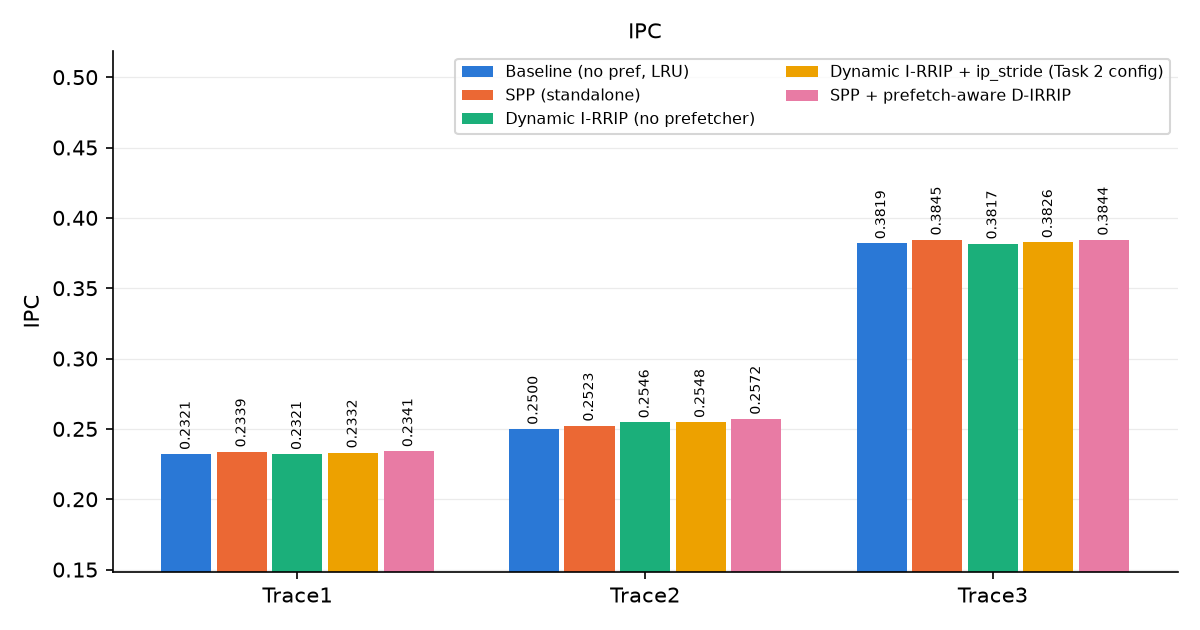
\includegraphics[width=0.8\textwidth]{ipc.png}
\caption{IPC.}
\end{figure}

\begin{figure}[H]
\centering
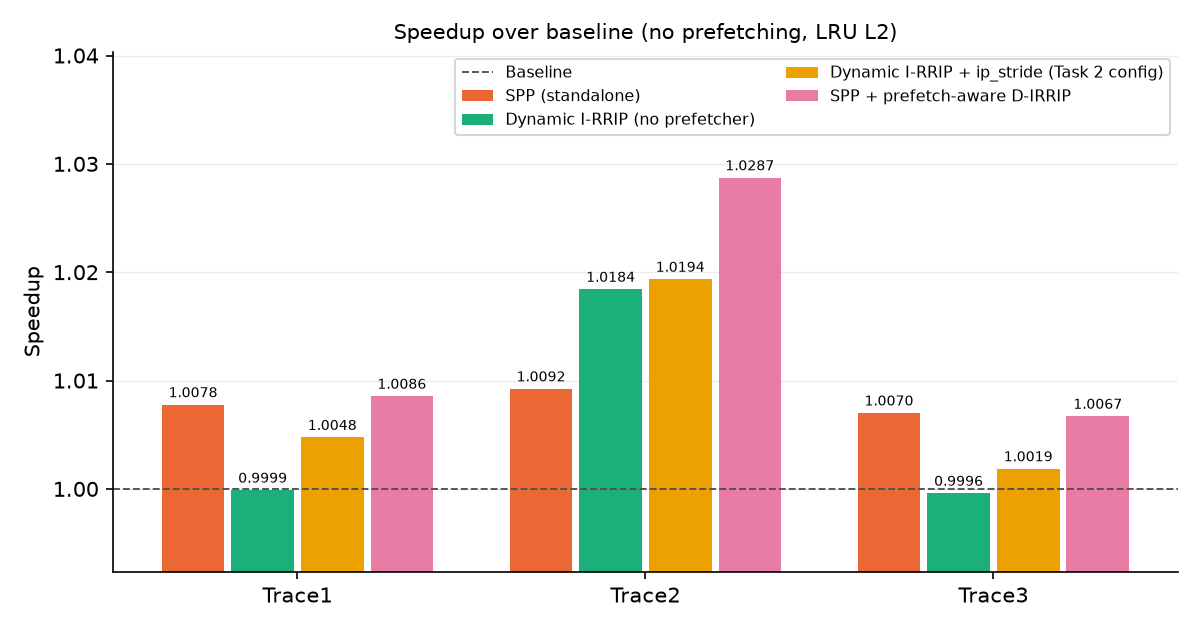
\includegraphics[width=0.8\textwidth]{speedup.png}
\caption{Speedup over the baseline.}
\end{figure}

\begin{figure}[H]
\centering
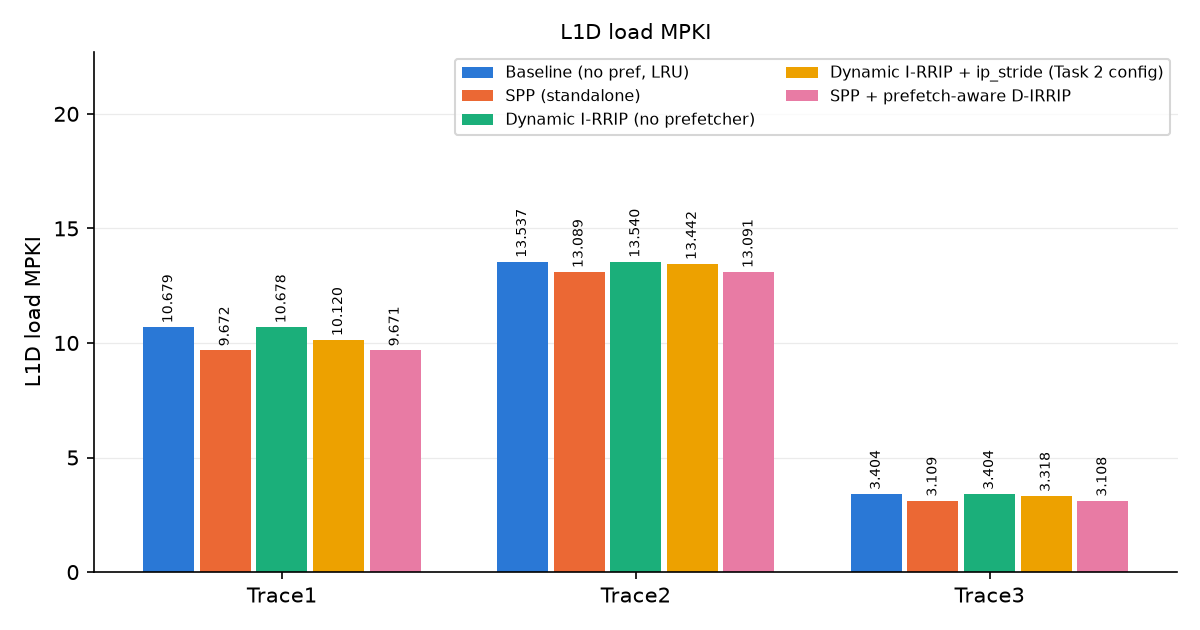
\includegraphics[width=0.8\textwidth]{l1d_mpki.png}
\caption{L1D load MPKI.}
\end{figure}

\begin{figure}[H]
\centering
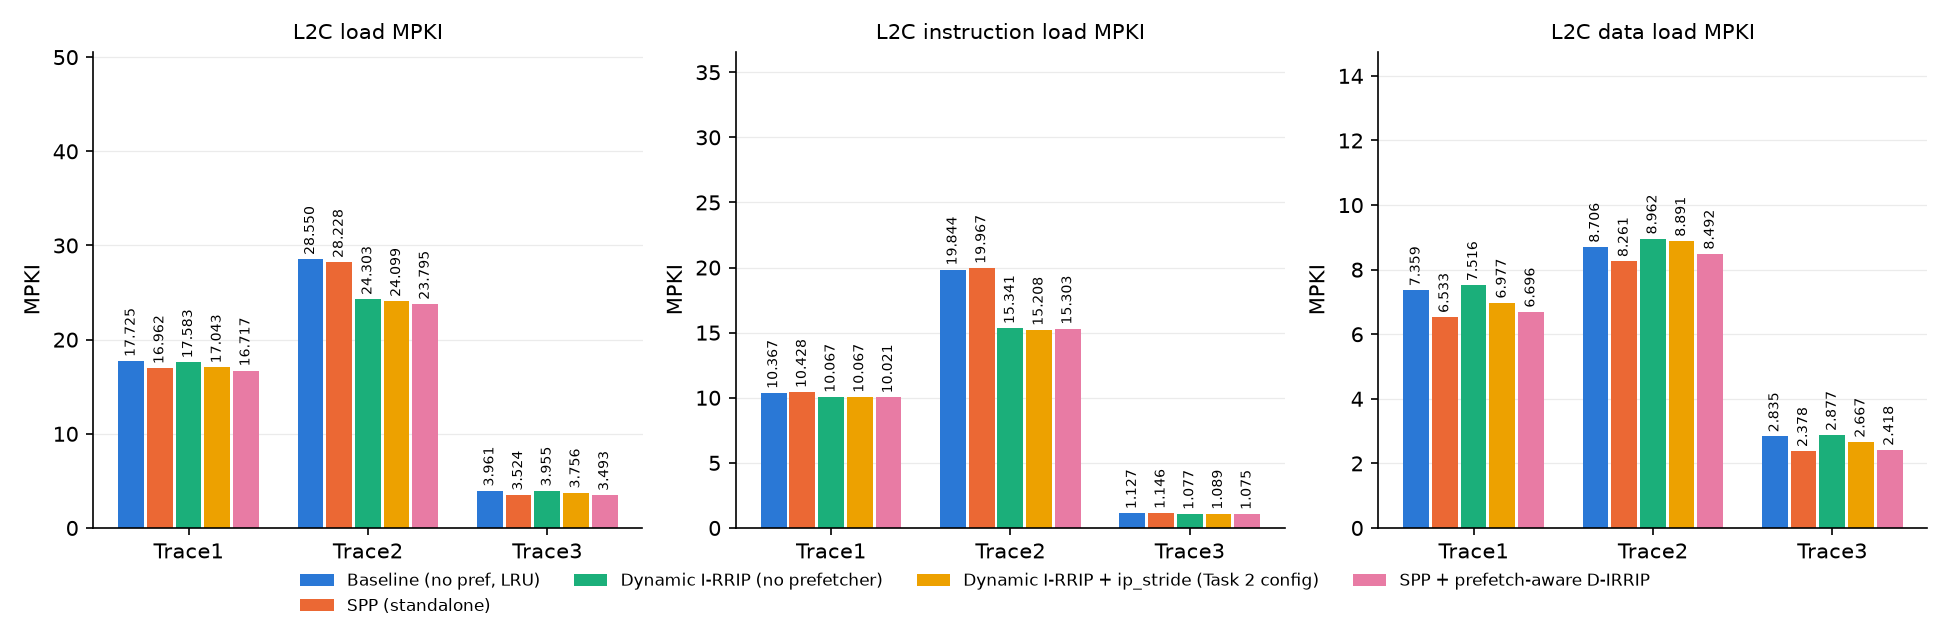
\includegraphics[width=\textwidth]{l2_mpki.png}
\caption{L2C total, instruction and data load MPKI.}
\end{figure}

\begin{figure}[H]
\centering
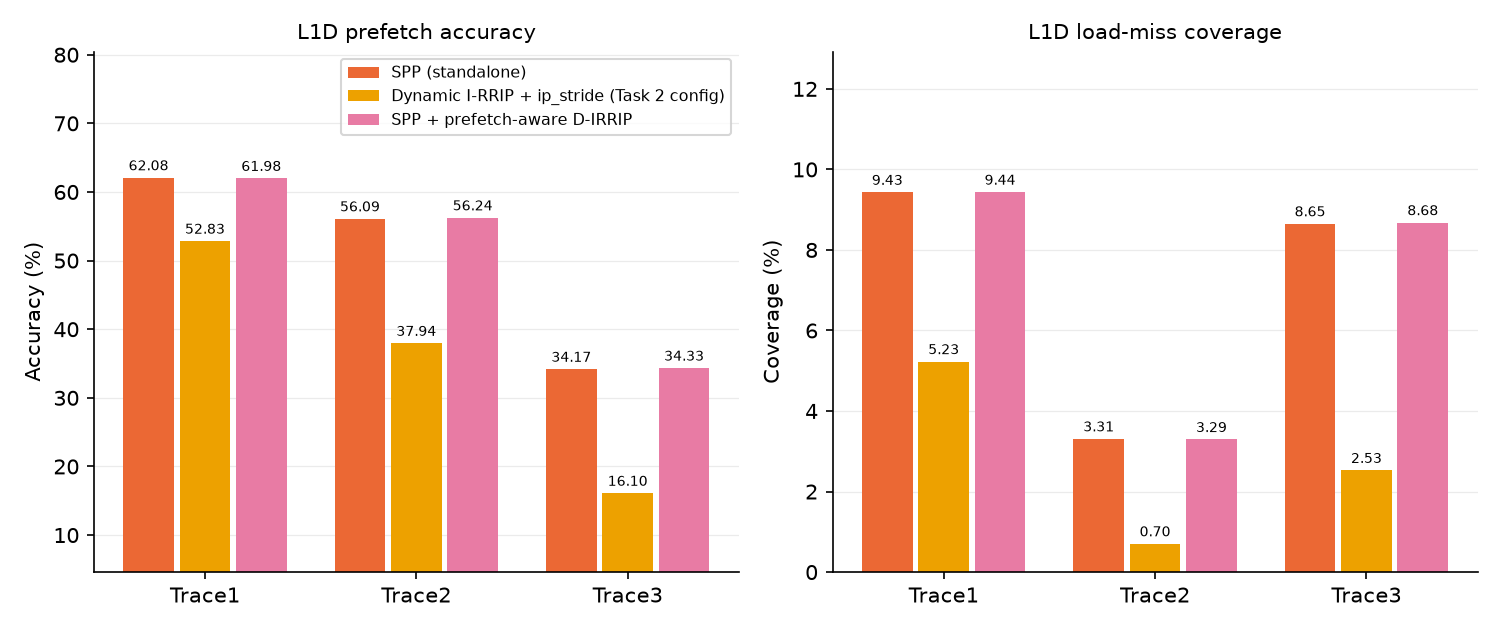
\includegraphics[width=\textwidth]{prefetch.png}
\caption{L1D prefetch accuracy and coverage.}
\end{figure}

\subsection*{2) Rationale for handling the prefetch packet}

SPP issues its prefetches with \texttt{FILL\_L1}, so a prefetched line is installed in the L1D as well as the L2. The program then reads it out of the L1D, and the L2 copy is frequently never touched again from the L2 side. Counters added to the policy measure this over the region of interest: of the prefetch fills into the follower sets, only 10.13\% (Trace1), 3.94\% (Trace2) and 14.70\% (Trace3) are ever used by a later non-prefetch access at the L2. These rates are a property of the Task 3 policy that produced them, so they are quoted as evidence that most prefetched lines do not need a demand-priority slot, not as a measurement of how Task 2 behaved.

The direct evidence that the two mechanisms interfere is in the results table itself. Under the Task 2 policy a prefetched line was inserted at RRPV 2, the same position as a demand data line. Running SPP on its own \emph{raises} L2 instruction MPKI above the baseline on all three traces: 10.3665 to 10.4284 on Trace1, 19.8440 to 19.9669 on Trace2, and 1.1265 to 1.1462 on Trace3. Prefetched data is displacing the instruction lines that I-RRIP exists to protect. Task 3 reverses this on all three traces, reaching 10.0211, 15.3027 and 1.0747, below the baseline in every case.

A \texttt{uint8\_t is\_pf[L2C\_SET][L2C\_WAY]} array records whether a line was filled by a prefetch and has not yet been used by a non-prefetch access. The test is \texttt{type == PREFETCH} exactly, so \texttt{PREFETCH\_TRANSLATION} and \texttt{TRANSLATION\_FROM\_L1D} are excluded, since those are page-walk traffic rather than SPP lines.

Figure~\ref{fig:rrpv} shows the resulting RRPV state machine of one L2 line.

% Every rule drawn below maps to replacement/dyn_irrip.l2c_repl:
%   power-on RRPV 3 (l2c_initialize_replacement); instruction fill RRPV 1 or 2;
%   prefetch fill in a follower set RRPV 3 with is_pf set; any other fill RRPV 2;
%   hit -> RRPV 0 unless a PREFETCH-type hit in a follower set; ageing and victim
%   order in l2c_find_victim. Geometry: states 20 mm wide, 2.8 cm apart.
\begin{figure}[H]
\centering
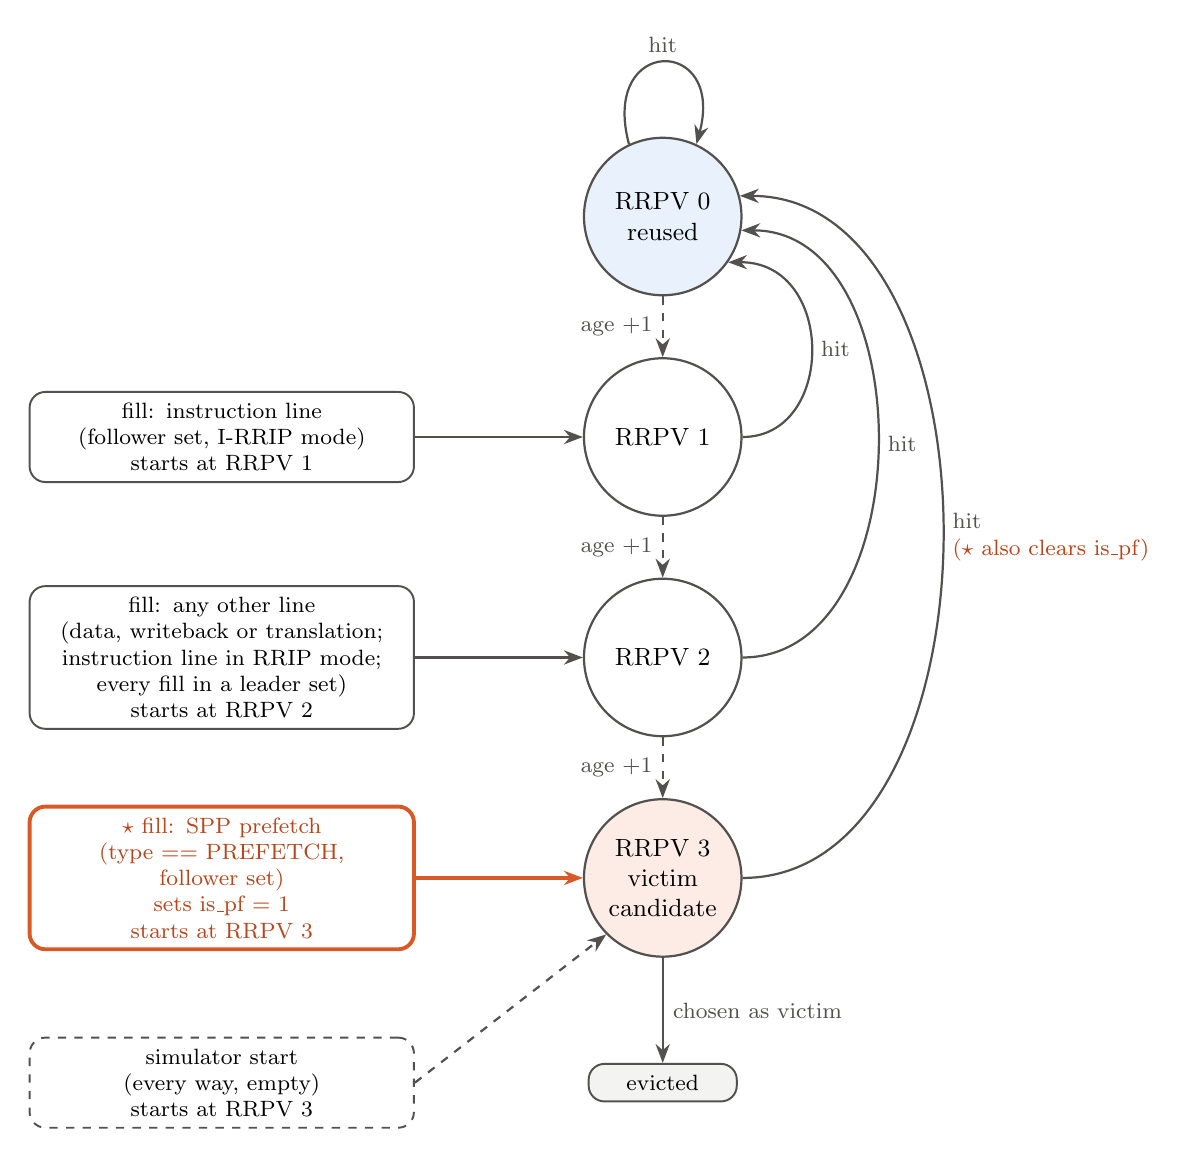
\begin{tikzpicture}[
    >={Stealth[length=2.4mm, width=1.8mm]},
    every node/.style={font=\small},
    state/.style={circle, draw=inkgrey, line width=0.8pt, minimum size=20mm, inner sep=0.5mm, align=center},
    fillbox/.style={rectangle, rounded corners=2mm, draw=inkgrey, line width=0.7pt, align=center,
                    text width=46mm, inner sep=4pt, font=\footnotesize},
    lbl/.style={font=\footnotesize, text=inkgrey},
    arr/.style={->, draw=inkgrey, line width=0.8pt},
  ]
  % the RRPV ladder: RRPV 0 = reused, RRPV 3 = next eviction candidate
  \node[state, fill=reusefill]  (r0) at (0, 0)    {RRPV 0\\reused};
  \node[state]                  (r1) at (0, -2.8) {RRPV 1};
  \node[state]                  (r2) at (0, -5.6) {RRPV 2};
  \node[state, fill=victimfill] (r3) at (0, -8.4) {RRPV 3\\victim\\candidate};
  \node[fillbox, fill=evictfill, text width=16mm] (ev) at (0, -11.0) {evicted};

  % ageing: only when a victim is needed and no line in the set is at RRPV 3
  \draw[arr, dashed] (r0) -- node[left, lbl] {age $+1$} (r1);
  \draw[arr, dashed] (r1) -- node[left, lbl] {age $+1$} (r2);
  \draw[arr, dashed] (r2) -- node[left, lbl] {age $+1$} (r3);
  \draw[arr] (r3) -- node[right, lbl] {chosen as victim} (ev);

  % promotion on a hit: nested arcs back to RRPV 0
  \draw[arr] (r1.east) .. controls (2.2, -2.8) and (2.2, -0.57) .. (r0.-35)
    node[pos=0.5, right, lbl] {hit};
  \draw[arr] (r2.east) .. controls (3.3, -5.6) and (3.3, -0.17) .. (r0.-10)
    node[pos=0.5, right, lbl] {hit};
  \draw[arr] (r3.east) .. controls (4.4, -8.4) and (4.4, 0.26) .. (r0.15)
    node[pos=0.5, right, lbl, align=left] {hit\\\textcolor{taskthreetext}{($\star$ also clears is\_pf)}};
  \draw[arr] (r0.115) .. controls (-0.8, 2.3) and (0.8, 2.3) .. (r0.65)
    node[pos=0.5, above, lbl] {hit};

  % where a line starts
  \node[fillbox] (f1) at (-5.6, -2.8)
    {fill: instruction line\\(follower set, I-RRIP mode)\\starts at RRPV 1};
  \node[fillbox] (f2) at (-5.6, -5.6)
    {fill: any other line\\(data, writeback or translation;\\instruction line in RRIP mode;\\every fill in a leader set)\\starts at RRPV 2};
  \node[fillbox, draw=taskthree, line width=1.4pt, text=taskthreetext] (f3) at (-5.6, -8.4)
    {$\star$ fill: SPP prefetch\\(type == PREFETCH, follower set)\\sets is\_pf = 1\\starts at RRPV 3};
  \node[fillbox, dashed] (st) at (-5.6, -11.0)
    {simulator start\\(every way, empty)\\starts at RRPV 3};

  \draw[arr] (f1) -- (r1);
  \draw[arr] (f2) -- (r2);
  \draw[arr, draw=taskthree, line width=1.4pt] (f3) -- (r3);
  \draw[arr, dashed] (st.east) -- (r3.-135);
\end{tikzpicture}

\vspace{0.8em}
\caption{RRPV state machine of one L2 line under the Task 3 policy (\texttt{replacement/dyn\_irrip.l2c\_repl}). Orange with $\star$ marks behaviour changed in Task 3; grey is unchanged Task 2 behaviour. In a follower set a line whose \texttt{is\_pf} bit is set is always at RRPV 3, which is why only the hit from RRPV 3 clears it.}
\label{fig:rrpv}
\end{figure}

\textbf{Insertion -- modified.} In the follower sets a prefetched line enters at RRPV 3 instead of RRPV 2. It still gets a full chance to be used before the set is next scanned, but it becomes the first candidate when a victim is needed, so it does not go on holding a slot ahead of an instruction line or a demand data line. (The fill itself still evicts a victim, as any fill does; \texttt{l2c\_find\_victim} does not look at the type of the incoming request. What changes is how long the prefetched line then occupies the set.) Together with the eviction preference below, this is what restores the instruction-MPKI reduction.

\textbf{Promotion -- modified.} In the follower sets, a hit whose \texttt{type} is \texttt{PREFETCH} no longer promotes the line to RRPV 0. A prefetch hitting a line the prefetcher itself installed is the prefetcher meeting its own work, not evidence that the program will reuse the line. Under the Task 2 rule a repeated prefetch stream could hold a dead line at RRPV 0 indefinitely, turning the policy into prefetcher-controlled LRU. The rule is applied to every prefetch hit in a follower set, including hits on lines a demand access originally brought in, because in both cases the prefetch itself carries no information about program reuse. A demand hit still promotes to RRPV 0 and clears the prefetch bit, because at that point the prefetch has been proven useful and the line deserves to be treated like any other reused line.

\textbf{Eviction -- modified.} The victim scan looks for a line at the maximum RRPV whose prefetch bit is still set before it considers any demand line. This applies in both follower branches, the I-RRIP one and the plain RRIP one, because an unused prefetched line is the cheapest thing to lose whether or not instruction prioritisation is currently active.

\textbf{Set-dueling counters -- modified.} Prefetch accesses are no longer counted in the leader-set instruction and data totals. The selector compares \texttt{(instruction accesses + instruction misses) / (all accesses + all misses)} against 0.25, and prefetch traffic is entirely on the data side, so counting it dilutes the instruction share and biases the selector toward plain RRIP on exactly the traces that benefit from I-RRIP. This changes what the selector observes, not how the leader sets themselves replace lines.

\textbf{Leader sets -- left as plain RRIP.} The three policy changes above are confined to the follower sets. Sets 0 to 31 keep plain RRIP insertion, promotion and eviction exactly as in Task 2, so the duel retains an unmodified control group.

\textbf{What was left alone.} The instruction and demand-data insertion positions (RRPV 1 under I-RRIP, RRPV 2 otherwise), the demand-hit promotion to RRPV 0, the ageing loop, the 32 leader sets and the 0.25 threshold are all unchanged from Task 2. The problem being fixed is specific to prefetched lines, so the rest of the policy had no reason to move, and holding it fixed makes the comparison against Task 2 a clean measurement of the prefetch handling alone.

\end{document}
